\subsection{Architettura delle informazioni}

\subsection{Design dell'interazione}

In figura \ref{blueprint} viene mostrato il blueprint dell'interazione
di CookApp. Si può notare come l'utente possa raggiungere le
funzionalità principali dell'applicazioni in bravi passi grazie ad
interfaccia semplice ed intuitiva. All'apertura dell'applicazione
l'utente si trova nella schermata ``Home page'' dalla quale può raggiungere 7
macrocategorie, le quali si diramano poi in diverse funzionalità che verranno
mostrate in seguito più nel dettaglio.\\
Si può inoltre notare dal blueprint che tutte le funzionalità della
sezione ``Lista della spesa''  sono raggruppate in un contenitore con la
denominazione ``SMARTWATCH''. Infatti quest'ultimo insieme di
funzionalità è disponibile anche nell'interfaccia per i dispositivi
smartwatch. Si assume che un utente utilizzi lo stesso account di
sistema tra i suoi dispositivi, i quali sincronizzano i loro dati
tramite il cloud condiviso.


\begin{landscape}
\label{fig:blueprint}
\begin{figure}[!h]
\centering
\fbox{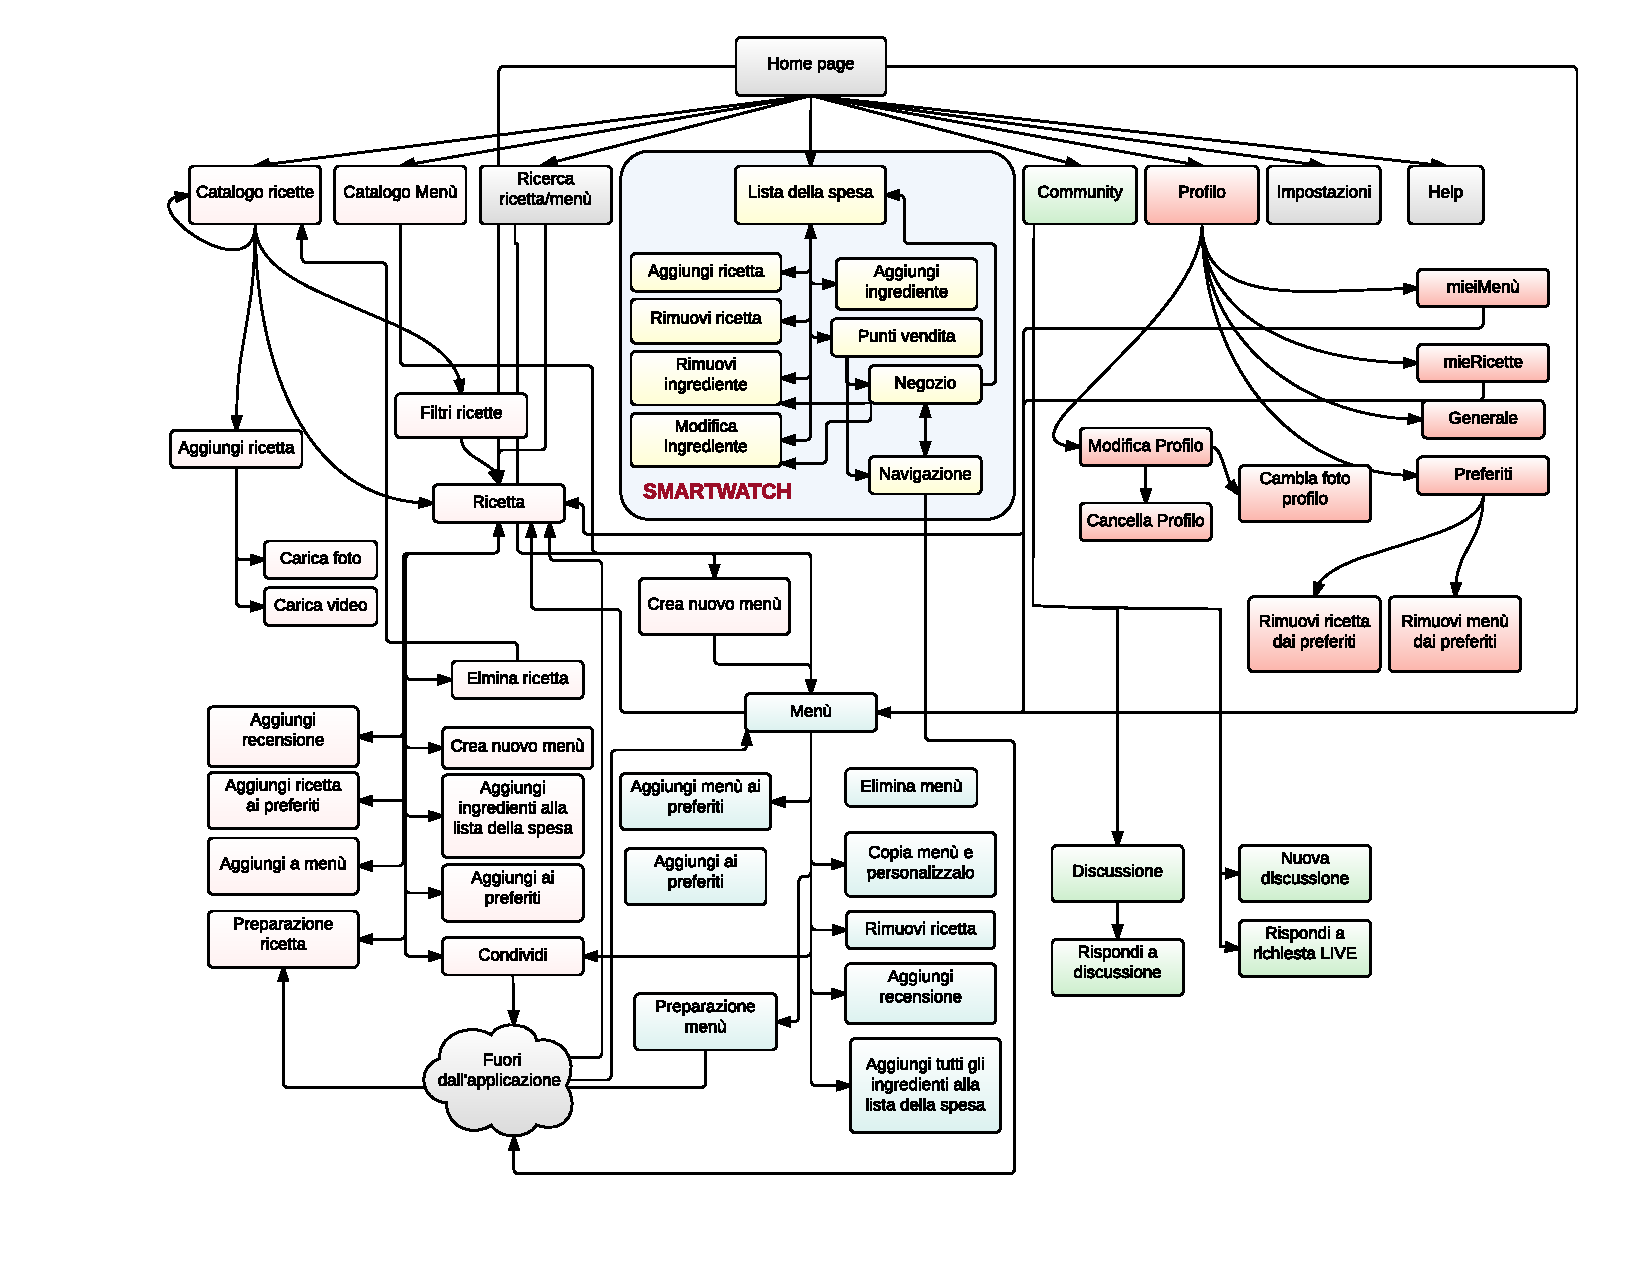
\includegraphics[width=\linewidth]{img/blueprint.pdf}}
\caption{Blueprint di CookApp}
\end{figure}
\end{landscape}

\subsection{Prototipo dell'interfaccia}
